\chapter{Aspectos económicos}
\label{cap:económicos}
\titlespacing{\section}{0em}{.75em}{.2em}
\titlespacing{\subsection}{0em}{.5em}{0em}
\section{Presupuesto del Proyecto}
El presupuesto para el diseño, desarrollo e implementación de la arquitectura IIoT para el parque eólico se ha estructurado en dos bloques principales: los costes de ingeniería y los costes correspondientes a la adquisición de licencias de software y amortización de infraestructura.

Los precios reflejados en el apartado de software corresponden a tarifas de catálogo industriales vigentes para el ecosistema \textit{SIMATIC WinCC}.

\subsection{Costes de Ingeniería (Mano de Obra)}
Para la estimación económica de las labores de desarrollo, se ha tomado como referencia el perfil de un Ingeniero Junior en la especialidad de Control, Automatización y Robótica. Tomando como base el salario especificado en el convenio colectivo de empresas de ingeniería para un nivel salarial 1 \cite{boe_convenio_ingenierias_2024}, se ha aplicado una tarifa de 12,00 € por hora para el ingeniero encargado del desarrollo técnico. Además, se ha considerado una tarifa de 16 € por hora para el director del TFM, quien supervisará y coordinará el proyecto.

El cálculo de horas (880 horas en total) refleja el volumen de dedicación requerido para un proyecto de esta envergadura (ver Tabla \ref{tab:presupuesto_mano_obra}).

\begin{table}[tbp]
\centering
\caption{Presupuesto de ingeniería y desarrollo técnico.}
\label{tab:presupuesto_mano_obra}
\resizebox{\textwidth}{!}{
\begin{tabular}{lccc}
\toprule
\textbf{Trabajador} & \textbf{Horas Estimadas} & \textbf{Tarifa (€)} & \textbf{Coste Total (€)} \\
\midrule
Ingeniero (Nivel 1) & 880 & 12.00 & 10.560,00 \\
Director de TFM & 20 & 16.00 & 320,00 \\
\midrule
\textbf{Total Mano de Obra} & \textbf{900} & & \textbf{10.880,00} \\
\bottomrule
\end{tabular}
}
\end{table}

\subsection{Licencias de Software WinCC}
El bloque tecnológico exige un alto nivel de inversión debido a la necesidad de gestionar una planta completa con un servidor SCADA masivo. La licencia principal \textit{WinCC RC} (que permite tanto ejecutar el entorno gráfico (\textit{Runtime}) como modificarlo (\textit{Configuration})) se ha dimensionado para soportar hasta 65.536 variables (\textit{tags}), cubriendo los datos simultáneos de todos los aerogeneradores. Por otro lado se utilizará la licencia de conectividad \textit{WinCC Connectivity Pack} para integrar el entorno SCADA con la nube, y la licencia de \textit{WinCC Cloud Connect} para habilitar la comunicación con la instancia virtualizada en AWS.

\begin{table}[tbp]
\centering
\caption{Presupuesto desglosado de licencias de software (Base y Upgrade), hardware e infraestructura.}
\label{tab:presupuesto_licencias_desglosado}
\resizebox{\textwidth}{!}{
\begin{tabular}{lcr}
\toprule
\textbf{Descripción del Software / Hardware} & \textbf{Cantidad} & \textbf{Coste Total (EUR)} \\
\midrule
SIMATIC WinCC RC (65536 tags) - Licencia Base & 1 & 14.200,00 \\
SIMATIC WinCC RC (65536 tags) - Upgrade a V8.1 & 1 & 2.300,00 \\
SIMATIC WinCC Cloud Connect - Licencia Base & 1 & 400,00 \\
SIMATIC WinCC Cloud Connect - Upgrade a V8.1 & 1 & 150,00 \\
SIMATIC WinCC Connectivity Pack - Licencia Base & 1 & 1.150,00 \\
SIMATIC WinCC Connectivity Pack - Upgrade a V8.1 & 1 & 450,00 \\
Amortización equipo de desarrollo (Estación base) & 1 & 1.000,00 \\
\midrule
\textbf{Total Software e Infraestructura} & & \textbf{19.650,00} \\
\bottomrule
\end{tabular}
}
\end{table}
\subsection{Infraestructura AWS}

El coste de la infraestructura en la nube se ha estimado en función del uso de una instancia EC2 de tipo \textit{t3.medium} . Este tipo de instancia ofrece un equilibrio adecuado entre recursos computacionales y coste, permitiendo alojar el entorno virtualizado necesario para la integración con el sistema SCADA. Como se observa en la Figura \ref{fig:aws_cost_estimation}, el coste mensual de esta instancia se ha calculado en base a las tarifas vigentes de AWS, considerando un uso continuo durante un periodo de aproximadamente 2 meses para cubrir la fase de desarrollo, pruebas e implementación del proyecto llegando a una estimación total de 19,87\$. 

\begin{figure}[tbp]
\centering
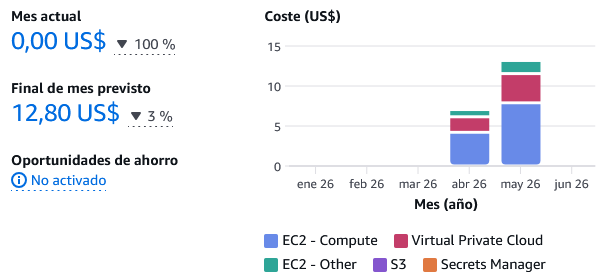
\includegraphics[width=\textwidth]{figuras/PrecioNube.png}
\caption{Estimación de costes para la instancia AWS EC2 t3.medium.}
\label{fig:aws_cost_estimation}
\end{figure}
\subsection{Resumen del Presupuesto y Coste Total}
La agregación de los costes de ingeniería, las licencias de software, la amortización de infraestructura local y el coste estimado de la infraestructura en AWS arroja la base imponible del proyecto (ver Tabla \ref{tab:presupuesto_total}).\vspace{0.5cm}

\begin{table}[htbp]
\centering
\caption{Resumen del presupuesto general del proyecto.}
\label{tab:presupuesto_total}
\begin{tabular}{p{10cm}p{3cm}}
\toprule
\textbf{Partida Presupuestaria} & \textbf{Importe (EUR)} \\
\midrule
Costes de Ingeniería (Mano de obra) & 10.880,00 \\
Costes de Software e Infraestructura & 19.650,00 \\
Coste estimado infraestructura AWS (2 meses) & 19,87 \\
\midrule
\textbf{Presupuesto Total General} & \textbf{30.549,87} \\
\bottomrule
\end{tabular}
\end{table}



